\chapter{Лабораторная работа №6. Основы работы с интерфейсом Ethernet}

\section{Структура пакета}
Для реализации приёма и передачи Ethernet пакета на ПЛИС необходимо рассмотреть структуру пакета. 

\subsection{Общая структура Ethernet пакета}

Базовая структура Ethernet кадра представлена на рисунке ~\ref{Ethernet_frame}. 

\begin{figure}[h]
	\centering
	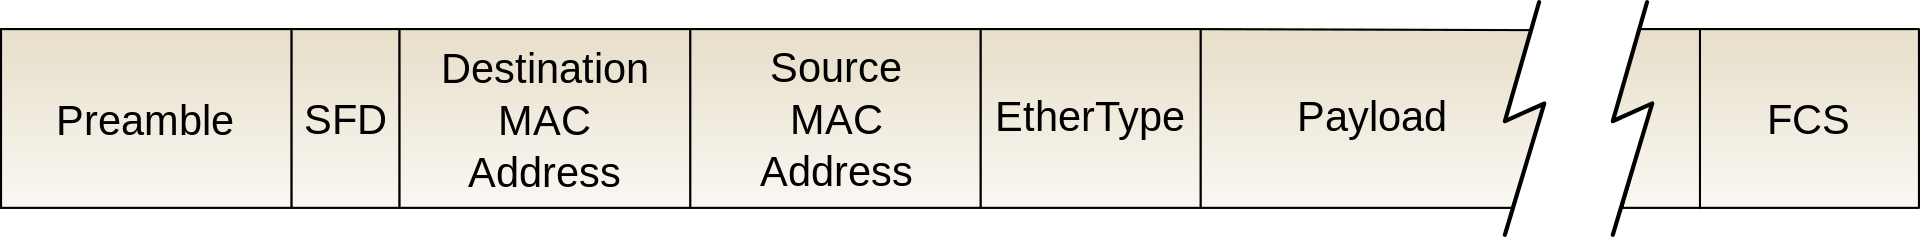
\includegraphics[width=0.9\textwidth]{image/Ethernet_frame}
	\caption{Общая структура Ethernet пакета}
	\label{Ethernet_frame}
\end{figure}

Рассмотрим подробно каждое поле пакета.

\begin{enumerate}
	\item Преамбула - 7 байт, ограничителя начала кадра - 1 байт. Ограничитель начала кадра (англ.Start frame delimiter, SFD) - это однобайтовое значение, которое отмечает конец преамбулы, является первым полем пакета Ethernet, и указывает начало кадра. SFD предназначен для разрыва битовой последовательности преамбулы и сигнализации о начале фактического кадра. Конкретное значение преамбулы и ограничителя начала кадра: 0x55, 0x55, 0x55, 0x55, 0x55, 0x55, 0x55, 0xD5.
	\item MAC адреса назначения – 6 байт, MAC адреса источника – 6 байт.
	\item Поле EtherType размером 2 байта используется для указания того, какой протокол инкапсулируют в полезной нагрузке кадра. Это же поле также используется для указания размера некоторых кадров Ethernet. Конкретное значение EtherType для четвёртой версия интернет-протокола (IPv4): 0x0800. Для ARP протокола(смотри 1.3.4) данное поле будет равно 0x0806.
	\item Полезная нагрузка - размер которой лежит в определённых границах. Минимальная полезная нагрузка составляет 42 байта при наличии тега 802.1Q и 46 байт при отсутствии. Когда фактическая полезная нагрузка меньше, соответственно добавляются байты заполнения. Максимальная полезная нагрузка - 1500 байта.  
	\item Последовательность проверки кадра (англ. Frame check sequence, FCS) — четырёхбайтное значение CRC, используемое для выявления ошибок передачи. Вычисляется отправляющей стороной и помещается в поле FCS. Принимающая сторона вычисляет данное значение самостоятельно и сравнивает с полученным(смотри 1.4).
\end{enumerate}

\subsection{Internet Protocol}
Протокол IP находится на межсетевом уровне стека протоколов TCP/IP. Функции протокола IP определены в стандарте RFC-791 следующим образом: “Протокол IP обеспечивает передачу блоков данных, называемых дейтаграммами, от отправителя к получателям, где отправители и получатели являются компьютерами, идентифицируемыми адресами фиксированной длины (IP-адресами). Протокол IP обеспечивает при необходимости также фрагментацию и сборку дейтаграмм для передачи данных через сети с малым размером пакетов”. Пакет сетевого уровня называется дейтаграммой. Дейтаграмма инкапсулируется непосредственно в полезную нагрузку Ethernet пакета(рис.~\ref{INC_IP}).
Структура дейтаграммы представлена на рисунке ~\ref{IP_protocol_paket}.

\begin{figure}[h]
	\centering
	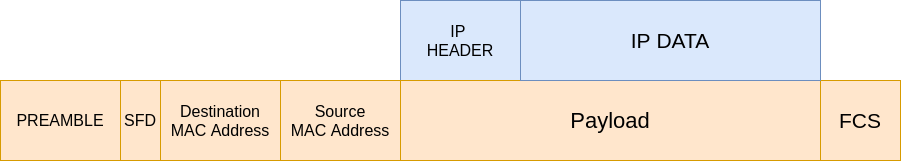
\includegraphics[width=0.9\textwidth]{image/IP}
	\caption{Инкапсуляция IP пакета}
	\label{INC_IP}
\end{figure}

\begin{figure}[h]
	\centering
	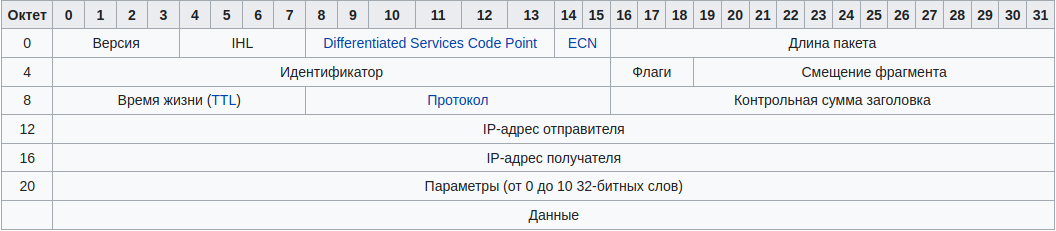
\includegraphics[width=0.9\textwidth]{image/IP-Protocol}
	\caption{Cтруктура IP пакета}
	\label{IP_protocol_paket}
\end{figure}

Протокол IP является ненадежным протоколом без установления соединения. Это означает, что протокол IP не подтверждает доставку данных, не контролирует целостность полученных данных и не производит операцию квитирования (handshaking) - обмена служебными сообщениями, подтверждающими установку соединения с узлом назначения и его готовность к приему данных. Протокол IP обрабатывает каждую дейтаграмму как независимую единицу, не имеющую связи ни с какими другими дейтаграммами в Интернет. После того, как дейтаграмма отправляется в сеть, ее дальнейшая судьба никак не контролируется отправителем (на уровне протокола IP). Если дейтаграмма не может быть доставлена, она уничтожается. Узел, уничтоживший дейтаграмму, может оправить по обратному адресу ICMP-сообщение о причине сбоя. Гарантию правильной передачи данных предоставляют протоколы вышестоящего уровня (например, протокол TCP), которые имеют для этого необходимые механизмы.

Рассмотрим подробно каждое поле дейтаграммы IPv4. 

\begin{enumerate}
	\item Версия — для IPv4 значение поля должно быть равно 4.
	\item IHL — (Internet Header Length) длина заголовка IP-пакета в 32-битных словах (dword). Именно это поле указывает на начало блока данных (англ. payload — полезный груз) в пакете. Минимальное корректное значение для этого поля равно 5.
	\item Биты типа обслуживания включены в заголовок дейтаграмм IPv4, чтобы отличать друг от друга различные типы IP-дейтаграмм (например, дейтаграммы с особыми требованиями к низкой задержке, высокой пропускной способности или надежности). К примеру, удобно отличать дейтаграммы, требующие реального времени (например, те, что исполь- зуются в IP-телефонии), от так называемого «оффлайнового» трафика (например, FTP).
	\item Длина пакета — (Total Length) длина пакета в октетах, включая заголовок и данные. Минимальное корректное значение для этого поля равно 20, максимальное — 65 535.
	\item Идентификатор — (Identification) значение, назначаемое отправителем пакета и предназначенное для определения корректной последовательности фрагментов при сборке пакета. Для фрагментированного пакета все фрагменты имеют одинаковый идентификатор.
	\item 3 бита флагов. Первый бит должен быть всегда равен нулю, второй бит DF (don’t fragment) определяет возможность фрагментации пакета и третий бит MF (more fragments) показывает, не является ли этот пакет последним в цепочке пакетов.
	\item Смещение фрагмента — (Fragment Offset) значение, определяющее позицию фрагмента в потоке данных. Смещение задается количеством восьмибайтовых блоков, поэтому это значение требует умножения на 8 для перевода в байты.
	\item Время жизни (TTL) — число маршрутизаторов, которые может пройти этот пакет. При прохождении маршрутизатора это число уменьшается на единицу. Если значение этого поля равно нулю, то пакет должен быть отброшен, и отправителю пакета может быть послано сообщение Time Exceeded (ICMP тип 11 код 0).
	\item Протокол — идентификатор сетевого протокола следующего уровня указывает, данные какого протокола содержит пакет, например, TCP, UDP, или ICMP (см. IANA protocol numbers и RFC 1700). Приведём значения данного поля для часто используемых протоколов: ICMP - 1, TCP -6, UDP - 17.
	\item Контрольная сумма заголовка. В протоколе IPv4 контрольная сумма рассчитывается только для заголовка пакета. Ниже представлен алгоритм расчёта контрольной суммы, а также численный пример. Для более подробного ознакомления с процедурой вычисления контрольной суммы в протоколах сетевого и транспортного уровня сети Интернет и
	вариантами ее реализации для различных языков программирования рекомендуется обратиться к RFC 1071.
	\item Параметры. Поля параметры расширяют заголовок. Они предназначены для
	исключительных случаев, поэтому информация об параметрах не включается в заголовок каждой дейтаграммы. Размер параметров составляет от нуля до десяти 32-битных слов.
	\item Данные (полезное содержимое). Наконец, обсуждение подошло к последнему и самому важному полю — ради него и создается дейтаграмма. Чаще всего поле данных IP-дейтаграммы содержит сегмент транспортного уровня (протоколы TCP или UDP), необходимый для ее доставки в место назначения. Однако поле данных может содержать и другие типы данных, такие как сообщения ICMP.
\end{enumerate}


Контрольная сумма заголовка передаваемого пакета IPv4 рассчитывается по следующему алгоритму:

\begin{enumerate}
	\item Заголовок разбивается на слова \begin{math} W_i \end{math}
	по 16 бит. При необходимости последнее слово заголовка дополняется нулями справа (биты заполнения), чтобы «выровнять» длину заголовка в битах кратно 16.
	\item Значение поля контрольной суммы, которому соответствует слово
	\begin{math} W_6 \end{math}, принимается равным нулю.
	\begin{displaymath} 
	W_s = 0000_\text{16}
	\end{displaymath}
	\item Полученные 16-битные слова \begin{math} W_i \end{math} поэлементно суммируются между собой, как двоичные числа с переносом в старшие разряды:
	\begin{displaymath} 
	W_s = \sum_{i} W_i
	\end{displaymath}
	\item В том случае, если результат сложения \begin{math} W_s \end{math} в двоичном представлении превышает по длине 16 бит, он разбивается на два 16-битных слова, которые складываются между собой. Например,
	\begin{displaymath} 
	\text{если } W_s = 2A4E3_\text{16}, \text{то } W_s  = 0002_\text{16} + A4E3_\text{16} = A4E5_\text{16}.
	\end{displaymath}
	\item В случае, если результат сложения \begin{math} W_s \end{math} снова превышает 16 бит, предыдущая операция повторяется.
	\item Находится двоичное поразрядное дополнение результата сложения, которое и записывается в поле контрольной суммы:
	\begin{displaymath} FFFF_\text{16} - W_s. \end{displaymath}
\end{enumerate}

Для примера рассмотрим расчет контрольной суммы заголовка IP-пакета, приведенного на рис. 1.3. Пакет записан в шестнадцатеричной системе счисления. Поле контрольной суммы выделено цветом и обнулено перед началом формирования передаваемого IP-пакета.

\begin{figure}[h]
	\centering
	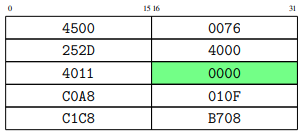
\includegraphics[width=0.4\textwidth]{image/check}
	\caption{Пример IP заголовка для расчёта контрольной суммы}
	\label{IP_protocol}
\end{figure}

\begin{enumerate}
	\item Разбиваем заголовок с обнуленным полем контрольной суммы на слова по 16 бит и суммируем полученные 16-битные слова между собой:
	\begin{displaymath} 
	4500_\text{16} + 0076_\text{16} + 252D_\text{16} + 4000_\text{16} + 
	4011_\text{16} + 
	\end{displaymath}
	\begin{displaymath} 
	+ \text{ }0000_\text{16} + C0A8_\text{16} + 010F_\text{16} + C1C8_\text{16} + B708_\text{16} = 3253B_\text{16}.
	\end{displaymath}
	\item Поскольку результат сложения в двоичном представлении превышает 16 разрядов (или 4 шестнадцатеричных цифры), разбиваем его на два слова
	по 16 бит каждое и снова их суммируем:
	\begin{displaymath} 
	0003_\text{16} + 253B_\text{16} = 253E_\text{16}.
	\end{displaymath}
	\item Находим контрольную сумму, как двоичное поразрядное дополнение
	результата сложения:
	\begin{displaymath} 
	FFFF_\text{16} - 253E_\text{16} = DAC1_\text{16}.
	\end{displaymath}
\end{enumerate}

Полученное число заносится в поле контрольной суммы заголовка IP пакета (рис. 1.3).
Проверка контрольной суммы при приеме IP-пакета производится по аналогичному алгоритму, отличаясь только тем, что в расчете участвует и контрольная сумма принятого IP-пакета. Если итоговое поразрядное двоичное дополнение полученной суммы равно 0x0000, то это говорит о корректности контрольной суммы.

Для примера проверим корректность контрольной суммы заголовка IP пакета, приведенного на рис. 1.3 с учетом значения поля контрольной суммы 0xDAC1.

\begin{enumerate}
	\item Суммируем все 16-битные слова заголовка между собой:
	\begin{displaymath} 
	4500_\text{16} + 0076_\text{16} + 252D_\text{16} + 4000_\text{16} + 4011_\text{16} + 
	\end{displaymath}
	\begin{displaymath} 
	+ \text{ }DAC1_\text{16} + C0A8_\text{16} + 010F_\text{16} + C1C8_\text{16} + B708_\text{16} = 3FFFC_\text{16}.
	\end{displaymath}
	\item Поскольку результат сложения превышает 16 бит, разбиваем его на
	два слова по 16 бит каждое и снова их суммируем:
	\begin{displaymath} 
	0003_\text{16} + FFFC_\text{16} = FFFF_\text{16}.
	\end{displaymath}
	\item Находим двоичное поразрядное дополнение результата сложения:
	\begin{displaymath} 
	FFFF_\text{16} - FFFF_\text{16} = 0000_\text{16}.
	\end{displaymath}
\end{enumerate}

Таким образом, мы проверили, что приведенная в пакете на рис 1.3 контрольная сумма верна.
Можно последнюю операцию поразрядного двоичного дополнения не
проводить. Тогда правильность контрольной суммы принятого IP-пакета будет подтверждаться результатом суммирования на втором шаге алгоритма проверки.

\subsection{User Datagram Protocol}
Протокол UDP (User Datagram Protocol, RFC-768) является одним из основных протоколов, расположенных непосредственно над IP. Он предоставляет прикладным процессам транспортные услуги, немногим отличающиеся от услуг протокола IP. Протокол UDP обеспечивает доставку дейтограмм, но не требует подтверждения их получения. Протокол UDP не требует соединения с удаленным модулем UDP ("бессвязный" протокол). К заголовку IP-пакета UDP добавляет поля порт отправителя и порт получателя, которые обеспечивают мультиплексирование информации между различными прикладными процессами, а также поля длина UDP-дейтограммы и контрольная сумма, позволяющие поддерживать целостность данных. Таким образом, если на уровне IP для определения места доставки пакета используется адрес, на уровне UDP - номер порта.

\begin{figure}[h]
	\centering
	\includegraphics[width=0.9\textwidth]{image/UDP}
	\caption{Инкапсуляция UDP пакета}
	\label{INC_UDP}
\end{figure}

\begin{figure}[h]
	\centering
	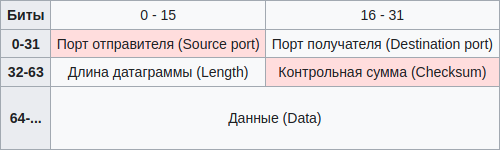
\includegraphics[width=0.6\textwidth]{image/udp}
	\caption{Структура UDP пакета}
	\label{UDP_protocol}
\end{figure}

\begin{figure}[h]
	\centering
	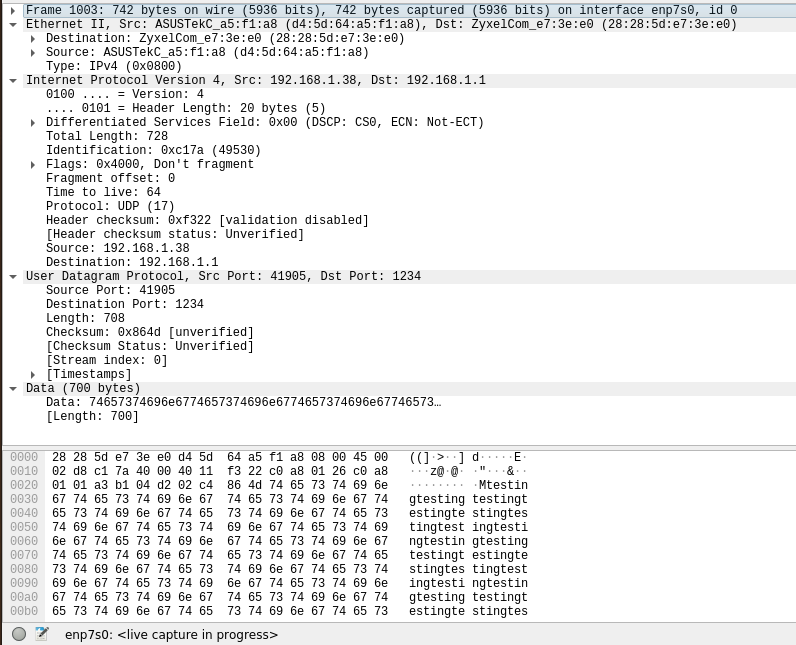
\includegraphics[width=0.9\textwidth]{image/example_UDP}
	\caption{Пример UDP пакета в Wireshark}
	\label{IP__exp_protocol}
\end{figure}

Структура UDP-сегмента, показанная на рис. 1.4, определена в стандарте RFC 768. Данные прикладного уровня размещаются в поле данных UDP-сегмента. Заголовок UDP-сегмента имеет только четыре поля, каждое из которых состоит из двух байт. Первые два байта указывают номер порта отправителя. Предполагается, что это значение задаёт порт, на который при необходимости будет посылаться ответ. В противном же случае, значение должно быть равным 0. Если хостом-источником является клиент, то номер порта будет, скорее всего, динамическим. Если источником является сервер, то его порт будет одним из «хорошо известных». Вторые два байта содержат порт получателя. Это поле уже является обязательным. Укажем, что номера портов позволяют хосту-получателю передавать данные приложения соответствующему процессу, запущенному на конечной системе получателе (то есть, предоставляют функцию демультиплексирования). 
В поле длина указана длина UDP-сегмента (заголовок плюс данные) в байтах. Явное указание значения в поле длины необходимо, поскольку размер поля данных может отличаться для каждого UDP-сегмента. Контрольная сумма UDP предназначена для обнаружения ошибок. Другими словами, контрольная сумма применяется для того, чтобы определить, произошло ли искажение битов UDP-сегмента (например, из-за помех в канале или при хранении на маршрутизаторе) в ходе перемещения от отправителя к получателю. Если сумма не сгенерирована передатчиком, то поле заполняется нулями. Поле не является обязательным для IPv4.

Рассмотрим пример вычисления контрольной суммы.

Основная идея состоит в том, что контрольная сумма UDP является дополнением до единицы к 16-битной сумме, вычисленной по «псевдозаголовку» IP и фактическим данным UDP. Псевдозаголовок IP - это адрес источника, адрес назначения, протокол (с добавлением нулевого байта) и длина UDP. Итак, чтобы взять пример этого короткого пакета, исходный IP-адрес - 152.1.51.27, а IP-адрес назначения - 152.14.94.75. Разделенные на 16-битные величины, это 0x9801, 0x331b и 0x980e, 0x5e4b. Если вы сложите их вместе, вы получите 0x1c175. Обратите внимание, что это переполняет 16-битное количество, но мы позаботимся об этом позже. Затем нужно добавить протокол и длину UDP. Для этого пакета используется протокол UDP, поэтому байт типа протокола - 17 или 0x11. Мы дополняем его нулем, чтобы получить 0x0011, а затем добавляем длину UDP, равную 0x000a (10 байт). Итак, 0x1c175 + 0x0011 + 0x000a = 0x1c190.

Теперь мы добавляем целую дейтаграмму UDP, рассматривая ее как 16-битные величины и пропуская контрольную сумму (пока мы не закончим ее вычисление!). Для этой дейтаграммы это 0x6262,0x000a, 0xa08f, 0x2694, поэтому, если мы добавим все это к нашей текущей сумме, мы получим 0x1c190 + 0xa08f + 0x2694 + 0x000a + 0x6262 = 0x2eb1f.

Теперь, чтобы преобразовать в 16-битную сумму с дополнением до единицы, мы просто обрабатываем нашу текущую сумму (0x2eb1f) как 32-битную величину и добавляем высокую половину к младшей половине. 0x0002 + 0xeb1f = 0xeb21. (Если бы все еще было переполнение, мы бы снова добавляли верхнюю и нижнюю половины до тех пор, пока не перестанет быть переполнение.) Теперь мы дополняем это количество (то есть переворачиваем все биты или выполняем операцию НЕ) и получаем значение 0x14de, что в точности соответствует контрольной сумме, указанной в пакете.

\begin{figure}[h]
	\centering
	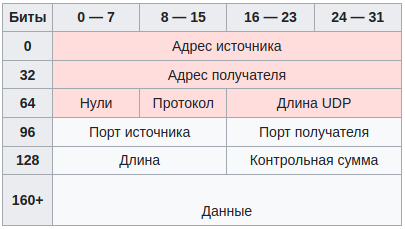
\includegraphics[width=0.6\textwidth]{image/pheader}
	\caption{UDP пакет с псевдозаголовком}
	\label{UDP_pheader}
\end{figure}


\subsection{Address Resolution Protocol}
ARP (англ. Address Resolution Protocol — протокол определения адреса) — протокол в компьютерных сетях, предназначенный для определения MAC-адреса по IP-адресу другого компьютера.

\begin{figure}[h]
	\centering
	\includegraphics[width=0.9\textwidth]{image/ARP}
	\caption{Инкапсуляция ARP пакета}
	\label{INC_ARP}
\end{figure}

Рассмотрим суть функционирования ARP на простом примере. Компьютер А (IP-адрес 10.0.0.1) и компьютер Б (IP-адрес 10.22.22.2) соединены сетью Ethernet. Компьютер А желает переслать пакет данных на компьютер Б, IP-адрес компьютера Б ему известен. Однако сеть Ethernet, которой они соединены, не работает с IP-адресами. Поэтому компьютеру А для осуществления передачи через Ethernet требуется узнать адрес компьютера Б в сети Ethernet (MAC-адрес в терминах Ethernet). Для этой задачи и используется протокол ARP. По этому протоколу компьютер А отправляет широковещательный запрос, адресованный всем компьютерам в одном с ним широковещательном домене. Суть запроса: «компьютер с IP-адресом 10.22.22.2, сообщите свой MAC-адрес компьютеру с МАС-адресом (напр. a0:ea:d1:11:f1:01)». Сеть Ethernet доставляет этот запрос всем устройствам в том же сегменте Ethernet, в том числе и компьютеру Б. Компьютер Б отвечает компьютеру А на запрос и сообщает свой MAC-адрес (напр. 00:ea:d1:11:f1:11) Теперь, получив MAC-адрес компьютера Б, компьютер А может передавать ему любые данные через сеть Ethernet.

\begin{figure}[h]
	\centering
	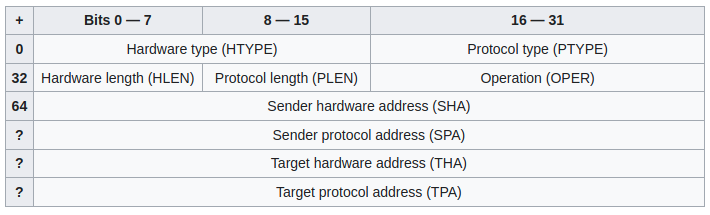
\includegraphics[width=0.9\textwidth]{image/arp}
	\caption{Cтруктура ARP пакета}
	\label{ARP_PROTOCOL}
\end{figure}

Рассмотри подробно каждое поле ARP пакета.

\begin{enumerate}
	\item Hardware type (HTYPE) - каждый канальный протокол передачи данных имеет свой номер, который хранится в этом поле. Например, Ethernet имеет номер 0x0001.
	\item Protocol type (PTYPE) - код сетевого протокола. Например, для IPv4 будет записано 0x0800.
	\item Hardware length (HLEN) - длина физического адреса в байтах. Адреса Ethernet имеют длину 6 байт (0x06).
	\item Protocol length (PLEN) - длина логического адреса в байтах. IPv4 адреса имеют длину 4 байта (0x04).
	\item Operation - код операции отправителя: 0x0001 в случае запроса и 0x0002 в случае ответа.
	\item Sender hardware address (SHA) - физический адрес отправителя.
	\item Sender protocol address (SPA) - логический адрес отправителя.
	\item Target hardware address (THA) - физический адрес получателя. Не требуется при запросе.
	\item Target protocol address (TPA) - логический адрес получателя.
\end{enumerate}

Ниже проиллюстрирована структура пакета, используемого в запросах и ответах ARP. В сетях Ethernet в этих пакетах используется EtherType 0x0806, и запросы рассылаются на широковещательный MAC-адрес — FF:FF:FF:FF:FF:FF. Отметим, что в структуре пакета, показанной ниже, в качестве SHA, SPA, THA и TPA условно используются 32-битные слова — реальная длина определяется физическим устройством и протоколом.

\begin{figure}[h]
	\centering
	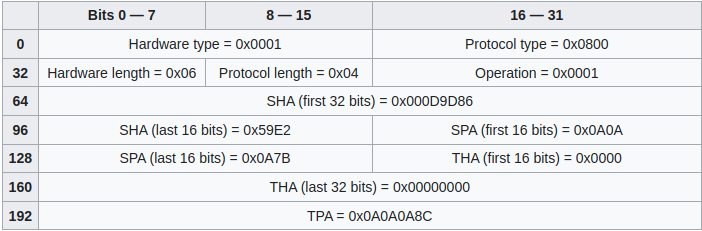
\includegraphics[width=0.9\textwidth]{image/arp2}
	\caption{Пример ARP пакета - запрос}
	\label{ARP_req}
\end{figure}

В ситуации, описанной выше, если узел с адресом 10.10.10.140 имеет MAC-адрес 00:09:58:D8:33:AA, то он отправит в ответ пакет, проиллюстрированный ниже. Заметим, что блоки адресов отправителя и получателя теперь поменяли значения (отправитель ответа теперь получатель запроса; получатель ответа — отправитель запроса). Кроме того, в ответе есть MAC-адрес узла 10.10.10.140 в поле физического адреса отправителя (SHA), а поле THA не пустое (одноадресный ответ).

Любой узел в той же сети, что и отправитель с получателем, тоже получит запрос (так как он широковещательный) и таким образом добавит в свой кэш информацию об отправителе. Ответ ARP направлен только источнику запроса ARP, поэтому ответ ARP не доступен другим узлам в сети.

\begin{figure}[h]
	\centering
	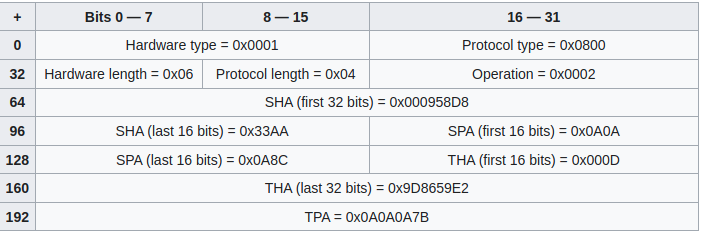
\includegraphics[width=0.9\textwidth]{image/arp1}
	\caption{Пример ARP пакета - ответ}
	\label{ARP_Response}
\end{figure}

Эффективность функционирования ARP во многом зависит от кэша ARP (ARP cache), который присутствует на каждом хосте. В кэше содержатся IP-адреса и соответствующие им аппаратные адреса.

\section{Media-independent interface}

\subsection{Gigabit Media-Independent Interface}
Gigabit Media-Independent Interface(GMII) — расширение стандарта MII (Media Independent Interface — независимый от среды передачи интерфейс) для гигабитных Ethernet-интерфейсов, обеспечивающий передачу данных между устройствами, реализующими подуровень Media Access Control (MAC) канального уровня с устройствами, реализующими физический уровень (PHY) модели OSI (например, как с оптическими интерфейсами 1000BASE-*X стандарта 802.3z, так и с медными интерфейсами 1000BASE-T* стандарта 802.3ab).

\begin{figure}[!ht]
	\centering
	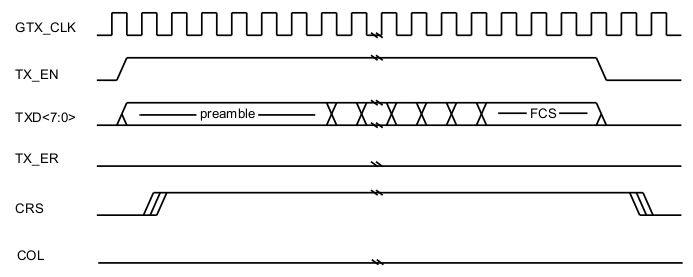
\includegraphics[width=0.9\textwidth]{image/GMII_transaction}
	\caption{Корректная передача кадра - GMII}
	\label{GMII_transaction}
\end{figure}

\begin{figure}[!ht]
	\centering
	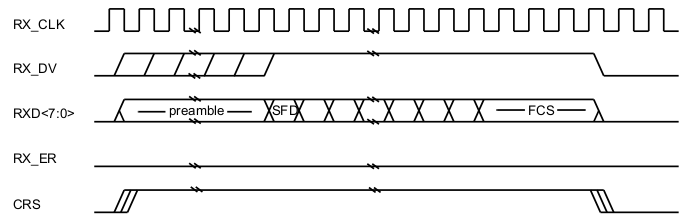
\includegraphics[width=0.9\textwidth]{image/GMII_RX}
	\caption{Корректный приём кадра - GMII}
	\label{GMII_RX}
\end{figure}

Описание сигналов данного интерфейса представлено в таблице 1. Интерфейс работает со скоростью до 1000 Мбит/с, реализован с использованием интерфейса данных с тактовой частотой 125 МГц с отдельными восьмибитными трактами данных для приема и передачи, обратно совместим со спецификацией MII, и может работать на скоростях 10 или 100 Мбит/с. 

Для работы данному интерфейсу необходимо два тактовых генератора. Выбор генератора зависит от того, работает ли PHY на гигабитных или 10/100 Мбит/с скоростях. Для гигабитной работы GTXCLK подается на PHY, и сигналы TXD, TXEN, TXER синхронизируются с этим. Для работы со скоростью 10 или 100 Мбит/с TXCLK предоставляется PHY и используется для синхронизации этих сигналов. Он работает на частоте 25 МГц для 100 Мбит/с или 2,5 МГц для соединений 10 Мбит/с. Приемник использует единственный тактовый сигнал, восстановленный из входящих данных. 

\subsection{Reduced Gigabit Media-Independent Interface}
Reduced Gigabit Media-Independent Interface(RGMII) - улучшенный интерфейс GMII. Улучшение состоит в том, что он использует меньшее количество выводов, необходимых для подключения PHY к MAC.
RGMII использует половину количества контактов данных, которые используются в интерфейсе GMII. Это сокращение достигается за счет:
\begin{enumerate}
	\item использования вместо восьми-битной шины данных четырёх-битную - теперь захват отчётов происходит как по переднему фронту тактового сигнала, так и по заднему;
	\item вместо двух отдельных сигналов валидности данных и сигнала ошибки используется один - они объединены вместе так, что по переднему фронту тактового сигнала происходит захват валидности данных, а по заднему фронту захват сигнала ошибки;
	\item исключения второстепенных сигналов определения несущей и индикации коллизий.
\end{enumerate} 

Уменьшение количества выводов снижает стоимость и сложность сетевого оборудования, особенно в контексте микроконтроллеров со встроенным MAC, FPGA, многопортовых коммутаторов или повторителей, а также наборов микросхем материнских плат ПК. 

\begin{figure}[!ht]
	\centering
	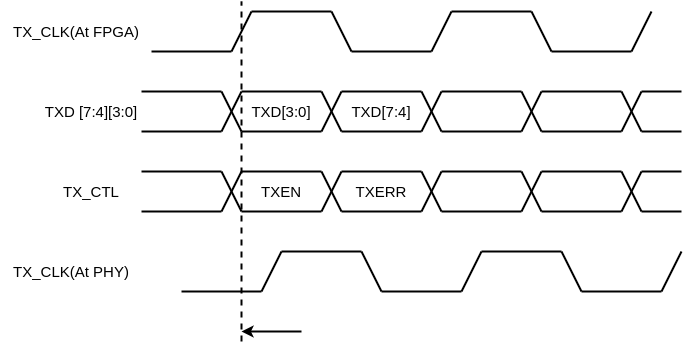
\includegraphics[width=0.8\textwidth]{image/TX_RGMII}
	\caption{Временные диаграммы линий передачи интерфейса RGMII}
	\label{TX_RGMII}
\end{figure}

\begin{figure}[!ht]
	\centering
	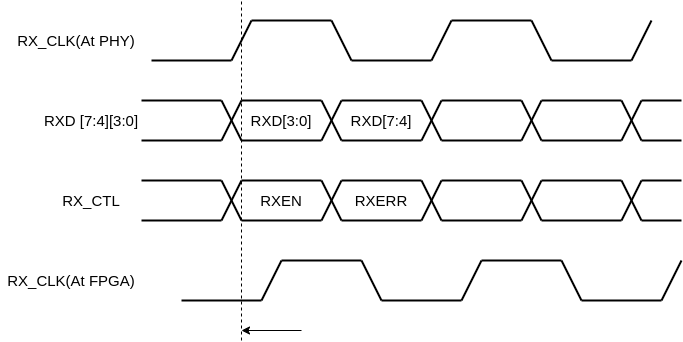
\includegraphics[width=0.8\textwidth]{image/RX_RGMII}
	\caption{Временные диаграммы линий приёма интерфейса RGMII}
	\label{TX_RGMII}
\end{figure}

\subsection{Serial Gigabit Media-Independent Interface}

\section{Практическая часть}

\begin{figure}[!ht]
	\centering
	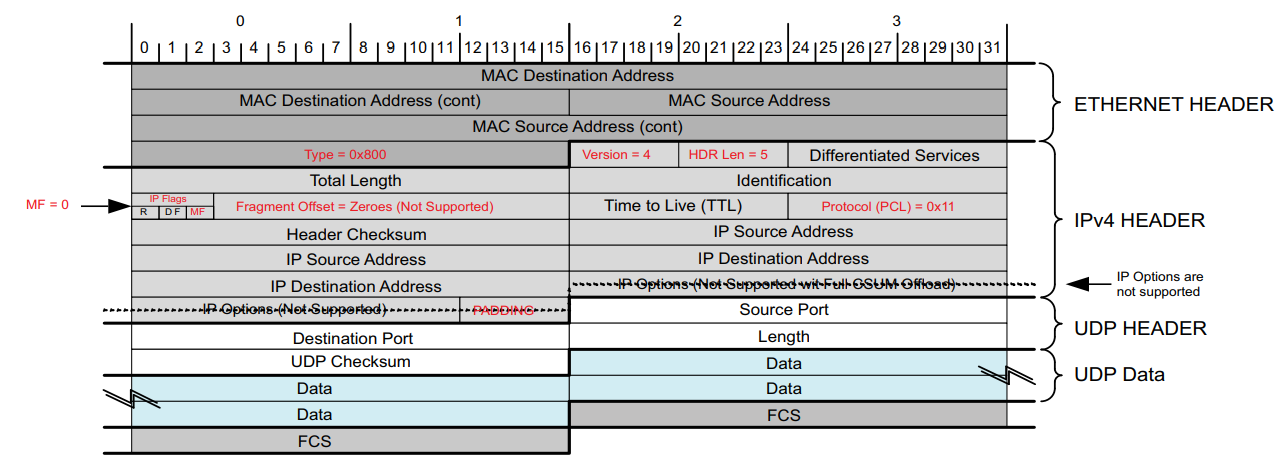
\includegraphics[width=0.8\textwidth]{image/eth_subsystem_frame.png}
	\caption{Временные диаграммы линий приёма интерфейса RGMII}
	\label{TX_RGMII}
\end{figure}

\section{Моделирование ядра}

\begin{Verbatim}[tabsize=4]
initial
begin
gtx_clk <= 1'b0;
#80000;
forever
begin
gtx_clk <= 1'b0;
#gtx_period;
gtx_clk <= 1'b1;
#gtx_period;
end
end
\end{Verbatim}

